\documentclass[12pt, a4paper]{article}
% \usepackage{ctex}
\usepackage[margin=1in]{geometry} 
\usepackage{amsmath,amsthm,amssymb}
\usepackage{bm}
\usepackage{cases}
\usepackage{graphicx}
\usepackage{hyperref}
\hypersetup{hidelinks}
\usepackage{amsfonts}
\usepackage{authblk}
\usepackage{mathrsfs}
\newcommand{\E}{\mathbb{E}}
\newcommand{\R}{\mathbb{R}}
\newcommand{\N}{\mathcal{N}}
\title{PRML Note\\C03 Linear Models for Regression}
\author{Yang Zhao}
\affil{Department of Automation, Tsinghua University}
\date{}

\begin{document}
    \maketitle
    %
    %  Chapter 1 Linear Basis Function Models
    %
    \begin{itemize}
        \item Given a training data set comprising $N$ observations $\{\bm{x}_n\}$, together with 
        corresponding target values $\{t_n\}$, the goal is to predict the value of $t$ for a new 
        value of $\bm{x}$.
        \item We can not only use the linear functions of the input variables, but also use the linear 
        combinations of a fixed set of nonlinear functions of the input variables, known as \textit{basis
         functions}. Such models are linear functions of the parameters and can be nonlinear with 
         respect to the input variables.
    \end{itemize}
    \section{Linear Basis Function Models}
    \begin{itemize}
        \item The simplest linear model for regression is
        \begin{align*}
            y(\bm{x},\bm{w})=w_0+w_1x_1+\cdots+w_Dx_D
        \end{align*}
        We can extend it by considering linear combinations of fixed nonlinear functions of the input
        variables, of the form
        \begin{equation}
            y(\bm{x},\bm{w})=w_0+\sum_{j=1}^{M-1}w_j\phi_j(\bm{x})
        \end{equation}
        where $\phi_j(\bm{x})$ are known as basis functions. We can also define an additional dummy basis
        function $\phi_0(\bm{x})=1$ so that
        \begin{equation}
            y(\bm{x},\bm{w})=\bm{w}^T\bm{\phi}(\bm{x})
        \end{equation}
        where $\bm{w}=(w_0,\cdots,w_{M-1})^T$ and $\bm{\phi}=(\phi_0,\cdots,\phi_{M-1})^T$.
        \item \textit{polynomial basis function}
        \begin{equation*}
            \phi_j(x)=x^j
        \end{equation*}
        One limitations of this basis functions is that they are global functions of the input variables, 
        so that changes in one region of input space affect all other regions. This can be resolved by 
        dividing the input space up into regions and fitting a different polynomial in each region, leading
        to \textit{spline functions}.
        \item \textit{Gaussian basis function}
        \begin{equation}
            \phi_j(x)=e^{-\frac{(x-\mu_j)^2}{2s^2}}
        \end{equation}
        where the $\mu_j$ govern the locations of the basis functions in input space and the $s$ governs 
        their spatial scale.
        \item \textit{sigmoidal basis function}
        \begin{equation}
            \phi_j(x)=\sigma\Big(\frac{x-\mu_j}{s}\Big)
        \end{equation}
        where $\sigma$ is the logistic sigmoid function defined by
        \begin{equation}
            \sigma(a)=\frac{1}{1+e^{-a}}
        \end{equation}
        \item We assume that the target variable $t$ is given by a deterministic function $y(\bm{x},\bm{w})$
        with additive Gaussian noise so that
        \begin{equation*}
            t=y(\bm{x},\bm{w})+\epsilon
        \end{equation*}
        where $\epsilon$ is a zero mean Gaussian random variable with precision $\beta$. Thus
        \begin{eqnarray}
            \label{eq:Gaussian}
            p(t|\bm{x},\bm{w},\beta)=\N (t|y(\bm{x},\bm{w}),\beta^{-1})
        \end{eqnarray}
        \item Consider a data set of inputs $\bm{X}=(\bm{x}_1,\bm{x}_2,\cdots,\bm{x}_N)$ with corresponding
        target values $\bm{t}=(t_1,t_2,\cdots,t_N)^T$, which are drawn independently from the distribution
        \ref{eq:Gaussian}, so we have
        \begin{equation*}
            p(\bm{t}|\bm{X},\bm{w},\beta)=\prod_{n=1}^N\N (t_n|\bm{w}^T\bm{\phi}(\bm{x}_n),\beta^{-1})
        \end{equation*}
        The gradient of the logliklihood function takes the form
        \begin{equation}
            \nabla lnp(\bm{t}|\bm{w},\beta)=\beta\sum_{n=1}^N(t_n-\bm{w}^T\bm{\phi}(\bm{x}_n))
            \bm{\phi}(\bm{x}_n)
        \end{equation}
        Setting this gradient to zero gives
        \begin{equation*}
            0=\sum_{n=1}^Nt_n\bm{\phi}(\bm{x}_n)-\Big(\sum_{n=1}^N\bm{\phi}(\bm{x}_n)\bm{\phi}(\bm{x}_n)^T
            \Big)\bm{w}
        \end{equation*}
        Solving for $\bm{w}$, we obtain
        \begin{eqnarray}
            \bm{w}_{ML}=(\bm{\Phi}^T\bm{\Phi})^{-1}\bm{\Phi}^T\bm{t}
        \end{eqnarray}
        where 
        \begin{equation*}
            \bm{\Phi}=\begin{pmatrix}
                \phi_0(\bm{x}_1) & \phi_1(\bm{x}_1) & \cdots & \phi_{M-1}(\bm{x}_1)\\
                \phi_0(\bm{x}_2) & \phi_1(\bm{x}_2) & \cdots & \phi_{M-1}(\bm{x}_2)\\
                \vdots & \vdots & \ddots & \vdots\\
                \phi_0(\bm{x}_N) & \phi_1(\bm{x}_N) & \cdots & \phi_{M-1}(\bm{x}_N)
            \end{pmatrix}
        \end{equation*}
        \item Considering the $w_0$, rewritten the error function, we have
        \begin{equation*}
            E_D(\bm{w})=\frac{1}{2}\sum_{n=1}^N(t_n-w_0-\sum_{j=1}^{M-1}w_j\phi_j(\bm{x}_n))
        \end{equation*}
        Setting the derivative with respect to $w_0$ equal to zero, and solving for $w_0$, we obtain 
        \begin{equation*}
            w_0=\bar{t}-\sum_{j=1}^{M-1}w_j\bar{\phi_j}
        \end{equation*}
        where we define
        \begin{align*}
            \bar{t}&=\frac{1}{N}\sum_{n=1}^Nt_n\\
            \bar{\phi_j}&=\frac{1}{N}\sum_{n=1}^N\phi_j(\bm{x}_n)
        \end{align*}
        Thus the bias $w_0$ compensates for the difference between the averages(over the training set) of 
        the target values and the weighted sum of the averages of the basis function values.
        \item We can also maximize the log likelihood function with respect to the noise precision parameters
        $\beta$, giving
        \begin{equation*}
            \frac{1}{\beta_{ML}}=\frac{1}{N}\sum_{n=1}^N(t_n-\bm{w}_{ML}^T\bm{\phi}(\bm{x}_n))^2
        \end{equation*}
        \item When $\bm{\Phi}^T\bm{\Phi}$ is close to singular, solving this problem directly will have 
        numerical difficulties. We can use \textit{singular value decomposition}, or SVD to address this 
        difficulties.
        \item \textit{LMS algorithm}. This is also known as \textit{least-mean-squares}. By applying the 
        technique of \textit{stochastic gradient descent}, we can update the $\bm{w}$
        \begin{align*}
            \bm{w}^{(t+1)}&=\bm{w}^{(t)}-\eta\nabla E_n\\
            &=\bm{w}^{(t)}-\eta(\bm{w}^{(t)T} \bm{\phi}_n-t_n)\bm{\phi}_n
        \end{align*}
        we can see how it works in figure \ref{fig:LMS}
        \begin{figure}[htbp]
            \begin{minipage}[t]{0.45\textwidth}
                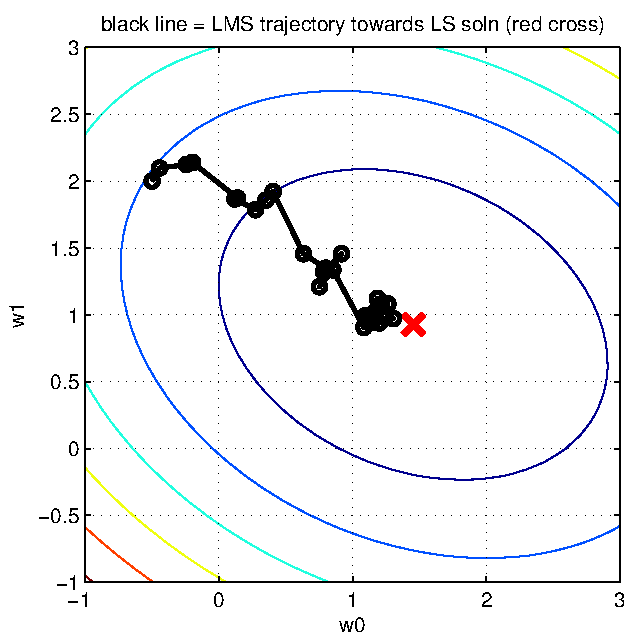
\includegraphics[width=0.8\textwidth]{figures/fig8_8a.pdf}
            \end{minipage}
            \hfill
            \begin{minipage}[t]{0.45\textwidth}
                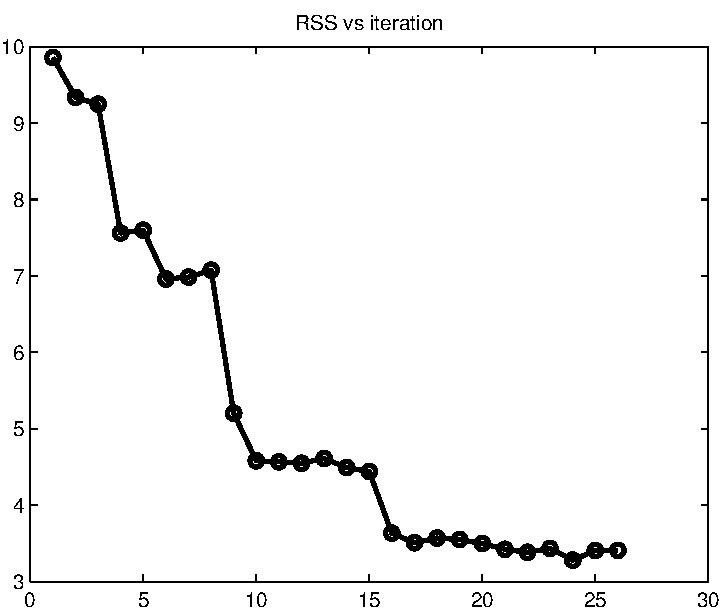
\includegraphics[width=1.0\textwidth]{figures/fig8_8b.pdf}
            \end{minipage}
            \label{fig:LMS}
            \caption{Illustration of LMS algorithm. Note that it doesn't decrease monotonically}
        \end{figure}
        \item By adding a regularization term to error function in order to control over-fitting, we get
        \begin{equation*}
            \frac{1}{2}\sum_{n=1}^N(t_n-\bm{w}^T\bm{\phi}(\bm{x}_n))^2+\frac{\lambda}{2}\bm{w}^T\bm{w}
        \end{equation*}
        This choice of regularizer is known in the ML literature as \textit{weight decay}. We obtain
        \begin{equation}
            \bm{w}=(\lambda\bm{I}+\bm{\Phi}^T\bm{\Phi})^{-1}\bm{\Phi}^T\bm{t}
        \end{equation}
        \item The problem of determining the optimal model complexity is then shifted from finding the
        appropriate number of basis functions to determining a suitable value of the regularization 
        coefficient $\lambda$.
        \item For multiple outputs, we could solve this problem by introducing a different set of basis 
        functions for each component of $\bm{t}$. But a more interesting and more common approach is to 
        use the same set of basis functions to model all of the components of target vector, so that
        \begin{equation}
            y(\bm{x},\bm{W})=\bm{W}^T\bm{\phi}(\bm{x})
        \end{equation}
        \item Consider a linear basis function regression model for a multivariate target variable 
        $\bm{t}$ having a Gaussian distribution of the form
        \begin{equation}
            p(\bm{t}|\bm{W},\bm{\Sigma})=\mathcal{N}(\bm{t}|y(\bm{x},\bm{W}),\bm{\Sigma})
        \end{equation}
        where $y(\bm{x},\bm{W})=\bm{W}^T\bm{\phi}(\bm{x})$, so the log-likelihood function is 
        \begin{equation*}
            lnp(\bm{T}|\bm{W},\bm{\Sigma})=\sum_{i=1}^N(\bm{t}_i-\bm{W}^T\phi(\bm{x}_i))^T
            \bm{\Sigma}^{-1}(\bm{t}_i-\bm{W}^T\phi(\bm{x}_i))
        \end{equation*}
        where
        \begin{equation*}
            \bm{T}=\begin{pmatrix}
                \bm{t}_1\\
                \bm{t}_2\\
                \vdots\\
                \bm{t}_N
            \end{pmatrix}=\begin{pmatrix}
                t_{11} & t_{12} & \cdots & t_{1K}\\
                t_{21} & t_{22} & \cdots & t_{2K}\\
                \vdots & \vdots & \ddots & \vdots\\
                t_{N1} & t_{N2} & \cdots & t_{NK}
            \end{pmatrix}
        \end{equation*}
        So, let
        \begin{align}
            \frac{\partial}{\partial{\bm{W}}}lnp(\bm{T}|\bm{W},\bm{\Sigma})&=\sum_{i=1}^N\phi(\bm{x}_i)
            \phi(\bm{x}_i)^T\bm{W}\bm{\Sigma}^{-1}-\phi(\bm{x}_i)\bm{t}_i\bm{\Sigma}^{-1}\nonumber\\
            &=\bm{\Phi}^T\bm{\Phi}\bm{W}\bm{\Sigma}^{-1}-\bm{\Phi}^T\bm{T}\bm{\Sigma}^{-1}\nonumber\\
            &=\bm{0}
        \end{align}
        we can get
        \begin{equation*}
            \bm{W}=(\bm{\Phi}^T\bm{\Phi})^{-1}\bm{\Phi}^T\bm{T}
        \end{equation*}
    \end{itemize}
    %
    %  Chapter 2 The Bias-Variance Decomposition
    %
    \section{The Bias-Variance Decomposition}
    \begin{itemize}
        \item Although the introduction of regularization terms can control over-fitting for models 
        with many parameters, this raises the question of how to determine a suitable value for the 
        regularization coefficient $\lambda$.
        \item Using an unbiased estimator is not always the best according to the bias-variance 
        trade-off.
        \item For the squared loss function, the optimal prediction is given by 
        \begin{equation*}
            h(\bm{x})=\E\lbrack t|\bm{x}\rbrack=\int tp(t|\bm{x})dt
        \end{equation*}
        Accordingt to Chapter 1, we known that
        \begin{eqnarray}
            \label{eq:LossDecomposition}
            \E\lbrack L\rbrack=\int(y(\bm{x})-h(\bm{x}))^2p(\bm{x})d\bm{x}+\iint(h(\bm{x})-t)^2p(t,\bm{x})
            dtd\bm{x}
        \end{eqnarray}
        The second term is independent of $y(\bm{x})$, representing the minimum achievable value of the 
        expected loss. For any given data set $\mathcal{D}$, we can get a prediction function 
        $y(\bm{x};\mathcal{D})$, and the average over the different data sets denotes by 
        $\E_{\mathcal{D}}(y(\bm{x};\mathcal{D}))$. So the first term in the equation 
        \ref{eq:LossDecomposition} can be rewritten by
        \begin{align}
            \label{eq:BVD}
            \textit{the first term}&=\int(y(\bm{x};\mathcal{D})-h(\bm{x}))^2
            p(\bm{x})d\bm{x}\nonumber\\
            &=\int(y(\bm{x};\mathcal{D})-\E_{\mathcal{D}}(y(\bm{x};\mathcal{D}))+
            \E_{\mathcal{D}}(y(\bm{x};\mathcal{D})-h(\bm{x}))^2)p(\bm{x})d\bm{x}\nonumber\\
            &=\{\E_{\mathcal{D}}(y(\bm{x};\mathcal{D}))-h(\bm{x})\}^2+\E_{\mathcal{D}}
            (y(\bm{x};\mathcal{D})-\E_{\mathcal{D}}\{y(\bm{x};\mathcal{D}))^2\}
        \end{align}
        \item the first term in equation \ref{eq:BVD} is called 
        \textit{the squared bias}, 
        which represents the extent to which the average prediction over all data sets differs from 
        the desired regression.
        \item the second term, called the \textit{variance}, measures the extent to which the solutions 
        for individual data sets vary around their average.
        \begin{figure}[htbp]
            \centering
            \label{fig:BVD}
            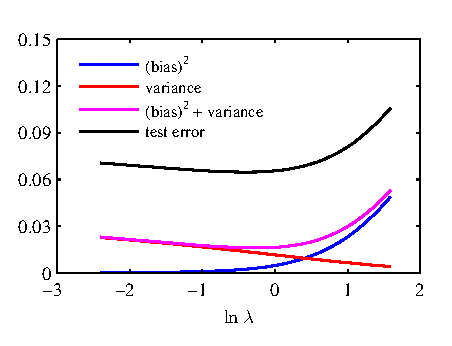
\includegraphics[width=0.5\textwidth]{figures/Figure3_6.eps}
            \caption{The bias-variance decomposition}
        \end{figure}
        \item The model with the optimal predictive capability is the one that leads to the best balance 
        between bias and variance.
        \item The bias-variance decomposition is based on averages with respect to ensembles of data sets, 
        whereas in practice we have only the single observed data set. And the larger data set can support 
        the larger capability of the model. So spliting the data set into many sets is not good for most 
        situations.
    \end{itemize}
    %
    %  Chapter 3 Bayesian Linear Regression
    %
    \section{Bayesian Linear Regression}
    \begin{itemize}
        \item Given the conjugate prior
        \begin{equation*}
            p(\bm{w})=\mathcal{N}(\bm{w}|\bm{m}_0,\bm{S}_0)
        \end{equation*}
        and the likelihood function
        \begin{equation*}
            p(\bm{t}|\bm{w})=p(\bm{t}|\bm{X},\bm{w},\beta)=\prod_{n=1}^N\N 
        (t_n|\bm{w}^T\bm{\phi}(\bm{x}_n),\beta^{-1})
        \end{equation*}
        So we can write the posterior distribution directly in the form
        \begin{equation*}
            p(\bm{w}|\bm{t})=\mathcal{N}(\bm{m}_N,\bm{S}_N)
        \end{equation*}
        where
        \begin{align*}
            \bm{m}_N&=\bm{S}_N(\bm{S}_0^{-1}\bm{m}_0+\beta\bm{\Phi}^T\bm{t})\\
            \bm{S}_N^{-1}&=\bm{S}_0^{-1}+\beta\bm{\Phi}^T\bm{\Phi}
        \end{align*}
        \item If data points arrive sequentially, then the posterior distribution at any stage acts as the
        prior distribution for the subsequent data point. By completing the square in the exponential, we 
        can obtain
        \begin{align*}
            \bm{S}_{N+1}^{-1}&=\bm{S}_N^{-1}+\beta\phi_{N+1}\phi_{N+1}^T\\
            \bm{m}_{N+1}&=\bm{S}_{N+1}(\bm{S}_N^{-1}\bm{m}_N+\beta\phi_{N+1}t_{N+1})
        \end{align*}
        \item Sometimes, we are not interested in the value of $\bm{x}$ itself but rather in making
        predictions of $t$ for new values of $\bm{x}$.
        \item The \textit{predictive distribution}
        \begin{equation*}
            p(t|\bm{x},\bm{t},\bm{X},\alpha,\beta)=\int p(t|\bm{x},\bm{w},\beta)
            p(\bm{w}|\bm{t},\bm{X},\alpha,\beta)d\bm{w}
        \end{equation*}
        where
        \begin{align*}
            p(t|\bm{x},\bm{w},\beta)&=\mathcal{N}(t|y(\bm{x},\bm{w}),\beta^{-1})\\
            p(\bm{w}|\bm{t},\bm{X},\alpha,\beta)&=\mathcal{N}(\bm{w}|\bm{m}_0,\bm{S}_0)
        \end{align*}
        So the predictive distribution takes the form
        \begin{equation*}
            p(t|\bm{x},\bm{w},\beta)=\mathcal{N}(t|\bm{m}_N^T(\phi(\bm{x})),\sigma_N^2(\bm{x}))
        \end{equation*}
        where
        \begin{equation*}
            \sigma_N^2(\bm{x})=\frac{1}{\beta}+\phi(\bm{x})^T\bm{S}_N\phi(\bm{x})
        \end{equation*}
        The first term represents the noise on the data whereas the second term reflects the uncertainty
        associated with the parameters $\bm{w}$.
        \item Assume we have already observed $N$ data points. By considering an additional 
        $(\bm{x}_{N+1},t_{N+1})$
        \begin{align*}
            \bm{S}_{N+1}^{-1}&=\bm{S}_N^{-1}+\beta\phi(\bm{x}_{N+1})\phi(\bm{x}_{N+1})^T\\
            \bm{m}_{N+1}&=\bm{S}_{N+1}(\bm{S}_N^{-1}\bm{m}_N+\phi(\bm{x}_{N+1})t_{N+1})
        \end{align*}
        So by completing the square in the exponential
        \begin{align*}
            \sigma_{N+1}^2(\bm{x})-\sigma_N^2(\bm{x})&=\frac{1}{\beta}+\phi(\bm{x})^T\bm{S}_N\phi(\bm{x})
            -\Big(\frac{1}{\beta}+\phi(\bm{x})^T\bm{S}_{N+1}\phi(\bm{x})\Big)\\
            &=\phi(\bm{x})^T(\bm{S}_{N+1}-\bm{S}_N)\phi(\bm{x})\\
            &=-\phi(\bm{x})^T\Big(\frac{\beta\bm{S}_N\phi(\bm{x}_{N+1})\phi(\bm{x}_{N+1})^T\bm{S}_N}
            {1+\beta\phi(\bm{x}_{N+1})^T\bm{S}_N\phi(\bm{x}_{N+1})}\Big)\phi(\bm{x})\\
            &\le 0
        \end{align*}
        because $\bm{S}_{N+1}-\bm{S}_{N}$ is negative definite matrix. So the second term in the predictive
        variance will go to zero.
        \item Considering the predictive mean, we obtain
        \begin{eqnarray}
            y(\bm{x},\bm{m}_M)=\bm{m}_N^T\phi(\bm{x})=\sum_{n=1}^N\beta\phi(\bm{x})^T\bm{S}_N\phi(\bm{x}_n)
            t_n
        \end{eqnarray}
        Thus the mean of the predictive at a point $\bm{x}$ is given by a linear combination of the 
        training set target variables $t_n$, so that we can write
        \begin{eqnarray}
            y(\bm{x},\bm{m}_N)=\sum_{n=1}^Nk(\bm{x},\bm{x}_n)t_n
        \end{eqnarray}
        where
        \begin{equation*}
            k(\bm{x},\bm{x}_n)=\beta\phi(\bm{x})^T\bm{S}_N\phi(\bm{x}_n)
        \end{equation*}
        is known as the \textit{smoother matrix} or the \textit{equivalent kernel}, which can also be 
        written as 
        \begin{equation*}
            k(\bm{x},\bm{z})=\psi(\bm{x})^T\psi(\bm{z})
        \end{equation*}
        where $\psi(\bm{x})=\beta^{1/2}\bm{S}_N^{1/2}\phi(\bm{x})$.
        \item We can see that $k(\bm{x},\bm{x}_n)$ can be weight of the linear combination and the data 
        points close to $\bm{x}$ are given higher weight than the data points further removed from $\bm{x}$.
        \item Note that the kernel function can be negative as well as positive, so although it satisfies
        a summation constraint, the corresponding predictions are not necessarily convex combinations of 
        the training set target variables.
    \end{itemize}
    %
    % Chapter 4 Bayesian Model Comparison
    %
    \section{Bayesian Model Comparison}
    \begin{itemize}
        \item Suppose we wish to compare a set of $L$ models $\{\mathcal{M}_i\}$ where $i=1,2,\cdots,L$. 
        Given a training set $\mathcal{D}$, we wish to caculate the posterior distribution $p(\mathcal{M}_i)$
        \begin{equation*}
            p(\mathcal{M}_i|\mathcal{D})\propto p(\mathcal{M}_i)p(\mathcal{D}|\mathcal{M}_i)
        \end{equation*}
        The prior allows us to express a preference for different models. Let us simply assume that all models
        are given equal prior probability. The interesting term is the \textit{model evidence} $p(\mathcal{D}
        |\mathcal{M}_i)$ which expresses the preference shown by the data for different models. The model 
        evidence is sometimes also called the \textit{marginal likelihood}. The ratio of model evidence 
        $p(\mathcal{D}|\mathcal{M}_i)/p(\mathcal{D}|\mathcal{M}_j)$ for two models is known as a 
        \textit{Bayes factor}.
    \end{itemize}
    %
    % Chapter 5 The Evidence Approximation
    %
    \section{The Evidence Approximation}
    \begin{itemize}
        \item In a fully Bayesian treatment of the linear basis function model, we would introduce prior 
        distributions over the hyperparameters $\alpha$ and $\beta$ and make predictions by marginalizing
        with respect to these hyperparameters as well as with respect to the parameters $w$, which is 
        analytically intractable. We can make an approximation in which we set the hyperparameters to specific
        values determined by maximizing the \textit{marginal likelihood function} obtained by first 
        integrating over the parameters $w$. This framework is known as \textit{empirical Bayes}, or 
        \textit{type 2 maximum likelihood}, or \textit{generalized maximum likelihood}, or \textit{evidence 
        approximation}.
        \item The predictive distribution is obtained by marginalizing over $\bm{w},\alpha,\beta$, so that
        \begin{equation}
            \label{eq:PredictiveDistribution}
            p(t|\bm{x},\bm{t},\bm{X})=\iiint p(t|\bm{x},\bm{w},\beta)p(\bm{w}|\bm{t},\bm{X},\alpha,\beta)
            p(\alpha,\beta|\bm{t},\bm{X})d\bm{w}d\alpha d\beta
        \end{equation}
        where 
        \begin{align*}
            p(t|\bm{x},\bm{w},\beta)&=\N(t|y(\bm{x},\bm{w}),\beta^{-1})\\
            p(\bm{w}|\bm{t},\bm{X},\alpha,\beta)&=\N(\bm{w}|\bm{m}_N,\bm{S}_N)\\
            \bm{m}_N&=\beta\bm{S}_N\bm{\Phi}^T\bm{t}\\
            \bm{S}_N^{-1}&=\alpha\bm{I}+\beta\bm{\Phi}^T\bm{\Phi}
        \end{align*}
        For posterior distribution $p(\alpha,\beta|\bm{t},\bm{X})$, we can simply assume the it is sharply
        peaked around values $\hat{\alpha}$ and $\hat{\beta}$, so
        \begin{equation*}
            p(t|\bm{x},\bm{t},\bm{X})\simeq p(t|\bm{x},\bm{t},\bm{X},\hat{\alpha},\hat{\beta})=
            \int p(t|\bm{x},\bm{w},\hat{\beta})p(\bm{w}|\bm{t},\bm{X},\hat{\alpha},\hat{\beta})d\bm{w}
        \end{equation*}
        and the posterior distribution for $\alpha$ and $\beta$ is given by
        \begin{equation*}
            p(\alpha,\beta|\bm{t},\bm{X})\propto p(\bm{t}|\alpha,\beta,\bm{X})p(\alpha,\beta)
        \end{equation*}
        If the prior is relatively flat, the value of $\hat{\alpha}$ and $\hat{\beta}$ are obtained by 
        maximizing the marginal likelihood function $p(\bm{t}|\alpha,\beta,\bm{X})$. We can both use the 
        analytially method by setting the derivative equal to zero and the expectation maximization algorithm.
        \item The marginal likelihood function $p(\bm{t}|\alpha,\beta,\bm{X})$ is obtained by integrating over
        the weight parameters $\bm{w}$, so that
        \begin{equation*}
            p(\bm{t}|\alpha,\beta,\bm{X})=\int p(\bm{t}|\bm{w},\beta,\bm{X})p(\bm{w}|\alpha)d\bm{w}
        \end{equation*}
        where
        \begin{align*}
            lnp(\bm{t}|\bm{w},\beta,\bm{X})&=\frac{N}{2}ln\beta-\frac{N}{2}ln(2\pi)-\beta E_D(\bm{w})\\
            E_D(\bm{w})&=\frac{1}{2}\Vert\bm{t}-\bm{\Phi}\bm{w}\Vert^2\\
            p(\bm{w}|\alpha)&=\N(\bm{w}|\bm{0},\alpha^{-1}\bm{I})
        \end{align*}
        \item We can write the evidence function in the form 
        \begin{equation*}
            p(\bm{t}|\alpha,\beta,\bm{X})=\Big(\frac{\beta}{2\pi}\Big)^{N/2}\Big(\frac{\alpha}{2\pi}
            \Big)^{M/2}\int e^{-E(\bm{w})}d\bm{w}
        \end{equation*}
        where 
        \begin{equation*}
            E(\bm{w})=\beta E_D(\bm{w})+\alpha E_W(\bm{w})=\frac{\beta}{2}\Vert\bm{t}-\bm{\Phi}\bm{w}
            \Vert^2+\frac{\alpha}{2}\bm{w}^T\bm{w}
        \end{equation*}
        we can complete the square over $\bm{w}$ giving 
        \begin{equation*}
            E(\bm{w})=E(\bm{m}_N)+\frac{1}{2}(\bm{w}-\bm{m}_N)^T\bm{A}(\bm{w}-\bm{m}_N)
        \end{equation*}
        where we have introduced
        \begin{align*}
            \bm{A}&=\alpha\bm{I}+\beta\bm{\Phi}^T\bm{\Phi}\\
            E(\bm{m}_N)&=\frac{\beta}{2}\Vert\bm{t}-\bm{\Phi}\bm{m}_N\Vert^2+\frac{\alpha}{2}\bm{m}_N^T
            \bm{m}_N\\
            \bm{m}_N&=\beta\bm{A}^{-1}\bm{\Phi}^T\bm{t}
        \end{align*}
        So the integral over $\bm{w}$ can now be evaluated as 
        \begin{align*}
            \int e^{-E(\bm{w})}d\bm{w}&=e^{-E(\bm{m}_N)}\int e^{-\frac{1}{2}(\bm{w}-\bm{m}_N)^T\bm{A}
            (\bm{w}-\bm{m}_N)}d\bm{w}\\
            &=e^{-E(\bm{m}_N)}(2\pi)^{M/2}\vert\bm{A}\vert^{-1/2}
        \end{align*}
        Thus we can obtain
        \begin{equation}
            \label{eq:EvidenceFunction}
            lnp(\bm{t}|\alpha,\beta,\bm{X})=\frac{M}{2}ln\alpha+\frac{N}{2}ln\beta-E(\bm{m}_N)-
            \frac{1}{2}ln\vert\bm{A}\vert-\frac{N}{2}ln(2\pi)
        \end{equation}
        \item Another way to get the equation \ref{eq:EvidenceFunction}. The likelihood function can
        be rewritten by
        \begin{equation*}
            p(\bm{t}|\bm{w},\beta,\bm{X})=\N(\bm{t}|\bm{\Phi}\bm{w},\beta^{-1}\bm{I}_N)
        \end{equation*}
        So, the result gives that
        \begin{equation*}
            p(\bm{t}|\alpha,\beta,\bm{X})=\N(\bm{0},\beta^{-1}\bm{I}_N+\alpha^{-1}\bm{\Phi}\bm{\Phi}^T)
        \end{equation*}
        Taking the log we obtain
        \begin{equation*}
            lnp(\bm{t}|\alpha,\beta,\bm{X})=-\frac{N}{2}ln(2\pi)-\frac{1}{2}ln\vert\beta^{-1}\bm{I}_N+
            \alpha^{-1}\bm{\Phi}\bm{\Phi}^T\vert-\frac{1}{2}\bm{t}^T(\beta^{-1}\bm{I}_N+\alpha^{-1}
            \bm{\Phi}\bm{\Phi}^T)^{-1}\bm{t}
        \end{equation*}
        Using the equation\ref{eq:DeterminantsExchange}, we have 
        \begin{align*}
            \vert\beta^{-1}\bm{I}_N+\alpha^{-1}\bm{\Phi}\bm{\Phi}^T\vert&=\beta^{-N}
            \vert\bm{I}_N+\beta\alpha^{-1}\bm{\Phi}\bm{\Phi}^T\vert\\
            &=\beta^{-N}\vert\bm{I}_M+\alpha^{-1}\bm{\Phi}^T\bm{\Phi}\vert\\
            &=\beta^{-N}\alpha^{-M}\vert\alpha\bm{I}_M+\beta\bm{\Phi}^T\bm{\Phi}\vert\\
            &=\beta^{-N}\alpha^{-M}\vert\bm{A}\vert
        \end{align*}
        and using the \textit{Woodbury matrix identity} introduced in Chapter2 appendix, we obtain
        \begin{align*}
            -\frac{1}{2}\bm{t}^T(\beta^{-1}\bm{I}_N+\alpha^{-1}\bm{\Phi}\bm{\Phi}^T)^{-1}\bm{t}&=
            -\frac{1}{2}\bm{t}^T\Big(\beta\bm{I}_N-\beta\bm{\Phi}(\alpha\bm{I}_M+\beta\bm{\Phi}^T
            \bm{\Phi})^{-1}\bm{\Phi}^T\beta\Big)\bm{t}\\
            &=-\frac{\beta}{2}\bm{t}^T\bm{t}+\frac{\beta^2}{2}\bm{t}^T\bm{\Phi}\bm{A}^{-1}\bm{\Phi}^T\bm{t}\\
            &=-\frac{\beta}{2}\bm{t}^T\bm{t}+\frac{1}{2}\bm{m}_N^T\bm{A}\bm{m}_N\\
            &=-\frac{\beta}{2}\Vert\bm{t}-\bm{\Phi}\bm{m}_N\Vert^2-\frac{\alpha}{2}\bm{m}_N^T\\
            &=-E(\bm{m}_N)
        \end{align*}
        and we have already got the same solutions as the equation \ref{eq:EvidenceFunction}.
        \item Maximizing the evidence function \ref{eq:EvidenceFunction} with respect to $\alpha$. First define
        the following eigenvector equation
        \begin{equation}
            \beta\bm{\Phi}^T\bm{\Phi}\bm{u}_i=\lambda_i\bm{u}_i
        \end{equation}
        Thus, we can know that the $\bm{A}$ has eigenvalues $\alpha+\lambda_i$. Because
        \begin{align*}
            \frac{d}{d\alpha}ln\vert\bm{A}\vert&=\frac{d}{d\alpha}ln\prod_i(\alpha+\lambda_i)\\
            &=\frac{d}{d\alpha}\sum_iln(\alpha+\lambda_i)\\
            &=\sum_i\frac{1}{\alpha+\lambda_i}
        \end{align*}
        Thus the stationary points of equation \ref{eq:EvidenceFunction} with respect to $\alpha$ satisfy
        \begin{equation}
            0=\frac{M}{2\alpha}-\frac{1}{2}\bm{m}_N^T\bm{m}_N-\frac{1}{2}\sum_i\frac{1}{\lambda_i+\alpha}
        \end{equation}
        So
        \begin{equation}
            \alpha\bm{m}_N^T\bm{m}_N=M-\alpha\sum_i\frac{1}{\lambda_i+\alpha}=\sum_i\frac{\lambda_i}
            {\lambda_i+\alpha}=\gamma
        \end{equation}
        which equals to
        \begin{equation}
            \alpha=\frac{\gamma}{\bm{m}_N^T\bm{m}_N}
        \end{equation}
        Note that this is an implicit solution for $\alpha$ not only because $\gamma$ depends on $\alpha$
        but also because the model $\bm{m}_N$ of the posterior distribution itself depends on the choice of
        $\alpha$, which means we have to use the iterative procedure to get the optimal $\alpha$.
        \item Maximizing the evidence function \ref{eq:EvidenceFunction} with respect to $\beta$. We note 
        that the eigenvalues $\lambda_i$ is proportional to $\beta$, and hence $d\lambda_i/d\beta=\lambda_i/
        \beta$ giving
        \begin{equation}
            \frac{d}{d\beta}ln\vert\bm{A}\vert=\frac{d}{d\beta}\sum_i(\lambda_i+\alpha)=\frac{1}{\beta}
            \sum_i\frac{\lambda_i}{\lambda_i+\alpha}=\frac{\gamma}{\beta}
        \end{equation}
        So
        \begin{equation}
            \frac{1}{\beta}=\frac{1}{N-\gamma}\sum_{n=1}^{N}(t_n-\bm{m}_N^T\phi(\bm{x}_n))^2
        \end{equation}
        which is also an implicit solution for $\beta$.
        \item The quantity $\gamma$ measures the effective tital number of well determined parameters.
    \end{itemize}
    %
    % Chapter 6 Limitations of Fixed Basis Functions
    %
    \section{Limitations of Fixed Basis Functions}
    \begin{itemize}
        \item The difficulty from the assumption that the basis functions $\phi_j(\bm{x})$ are fixed before 
        the training data set is observed. And the number of the basis functions needs to grow rapidly, often
        exponentially, with the dimensionality of the input space.
        \item The data vector typically lie close to a nonlinear manifold whose intrinsic dimensionality is 
        small.
        \item Target variables may have significant dependence on only a small number of possible directions
        within the data manifold.
    \end{itemize}
    %
    % Chapter 7 Appendix
    %
    \section{Appendix}
    \begin{itemize}
        \item \textit{The matrix identity for the sequential data}
        \begin{equation}
            \label{eq:MIforSD}
            (\bm{M}+\bm{v}\bm{v}^T)^{-1}=\bm{M}^{-1}-\frac{(\bm{M}^{-1}\bm{v})(\bm{v}^T\bm{M}^{-1})}
            {1+\bm{v}^T\bm{M}^{-1}\bm{v}}
        \end{equation}
        \item If $\bm{A}$ and $\bm{B}$ are matrices of size $N\times M$, then
        \begin{equation}
            \label{eq:DeterminantsExchange}
            \vert\bm{I}_N+\bm{A}\bm{B}^T\vert=\vert\bm{I}_M+\bm{A}^T\bm{B}\vert
        \end{equation}
        a useful special case is 
        \begin{equation*}
            \vert\bm{I}_N+\bm{a}\bm{b}^T\vert=1+\bm{a}^T\bm{b}
        \end{equation*}
        To prove the equation \ref{eq:DeterminantsExchange}, we notice that
        \begin{align*}
            \begin{bmatrix}
                \bm{I}_N & \bm{0} \\
                \bm{A}^T & \bm{I}_M
            \end{bmatrix}\begin{bmatrix}
                \bm{I}_N & \bm{B}\\
                -\bm{A}^T & \bm{I}_M
            \end{bmatrix}&=\begin{bmatrix}
                \bm{I}_N & \bm{B}\\
                \bm{0} & \bm{I}_M+\bm{A}^T\bm{B}
            \end{bmatrix}\\
            \begin{bmatrix}
                \bm{I}_N & \bm{B}\\
                -\bm{A}^T & \bm{I}_M
            \end{bmatrix}\begin{bmatrix}
                \bm{I}_N & \bm{0} \\
                \bm{A}^T & \bm{I}_M
            \end{bmatrix}&=\begin{bmatrix}
                \bm{I}_N+\bm{B}\bm{A}^T & \bm{B}\\
                \bm{0} & \bm{I}_M
            \end{bmatrix}
        \end{align*}
        So we have 
        \begin{equation*}
            det\begin{bmatrix}
                \bm{I}_N & \bm{B}\\
                \bm{0} & \bm{I}_M+\bm{A}^T\bm{B}
            \end{bmatrix}=det\begin{bmatrix}
                \bm{I}_N+\bm{B}\bm{A}^T & \bm{B}\\
                \bm{0} & \bm{I}_M
            \end{bmatrix}
        \end{equation*}
        which equals to
        \begin{equation*}
            \vert\bm{I}_M+\bm{A}^T\bm{B}\vert=\vert\bm{I}_N+\bm{B}\bm{A}^T\vert=
            \vert\bm{I}_N+\bm{A}\bm{B}^T\vert
        \end{equation*}
        where we use the result $det\bm{A}=det\bm{A}^T$.
    \end{itemize}
\end{document}